\documentclass{utarticle}
\PassOptionsToPackage{quiet}{fontspec}
\usepackage{ctex}
\usepackage{gezhu}
\usepackage{xcolor}
\usepackage{zhnumber}
\usepackage{amsmath}
\usepackage[dvipdfmx]{graphicx}
\usepackage[dvips]{adjustbox}
\usepackage{lscape}
% 背景图片
\usepackage{eso-pic}


% 文档类: utarticle
% 编译方式: uplatex main && dvipdfmx main


% 重定义section,subsection的计数器样式:
% 定义一个命令用于将阿拉伯数字映射到中文繁体
\newcommand{\tradnum}[1]{%
  \ifcase#1\relax%
  \or 壹% 1
  \or 贰% 2
  \or 叁% 3
  \or 肆% 4
  \or 伍% 5
  \or 陆% 6
  \or 柒% 7
  \or 捌% 8
  \or 玖% 9
  \or 拾% 10
  \else 未定义\fi% 其他情况
}
\renewcommand{\thesection}{\tradnum{\arabic{section}}}
\def\link{\raise2pt\hbox{.}\;\raise.2pt\hbox{{-}{-}}\;\raise2pt\hbox{.}}
\renewcommand{\thesubsection}{\thesection\;\link\zhnum{subsection}}
% 重定义图片的引入设置,添加一个旋转
\let\oldincludegraphics\includegraphics
\renewcommand{\includegraphics}[2][scale=1]{\oldincludegraphics[#1, angle=90]{#2}}
% 公式编号旋转90度
% \renewcommand{\theequation}{\rotatebox{90}{\arabic{equation}}}
% footnote的mark设置
\renewcommand{\thefootnote}{\textcolor{red}{\textcircled{\tiny\arabic{footnote}}}}
% 重新定义一个类似align的环境
\newenvironment{ralign}[1][.2\linewidth]{%
    \leavevmode\newline 
	\begin{adjustbox}{angle=90, center}
	\minipage{#1}
    \begin{center}$
    \begin{aligned}%
}{%
    \end{aligned}
    \hfill(\theequation)
    $\end{center}
    \endminipage
	\end{adjustbox}
}
\newcommand{\scale}[2]{%
    \scalebox{#1}[#1]{#2}}



\begin{document}
\AddToShipoutPictureBG*{%
    \AtPageLowerLeft{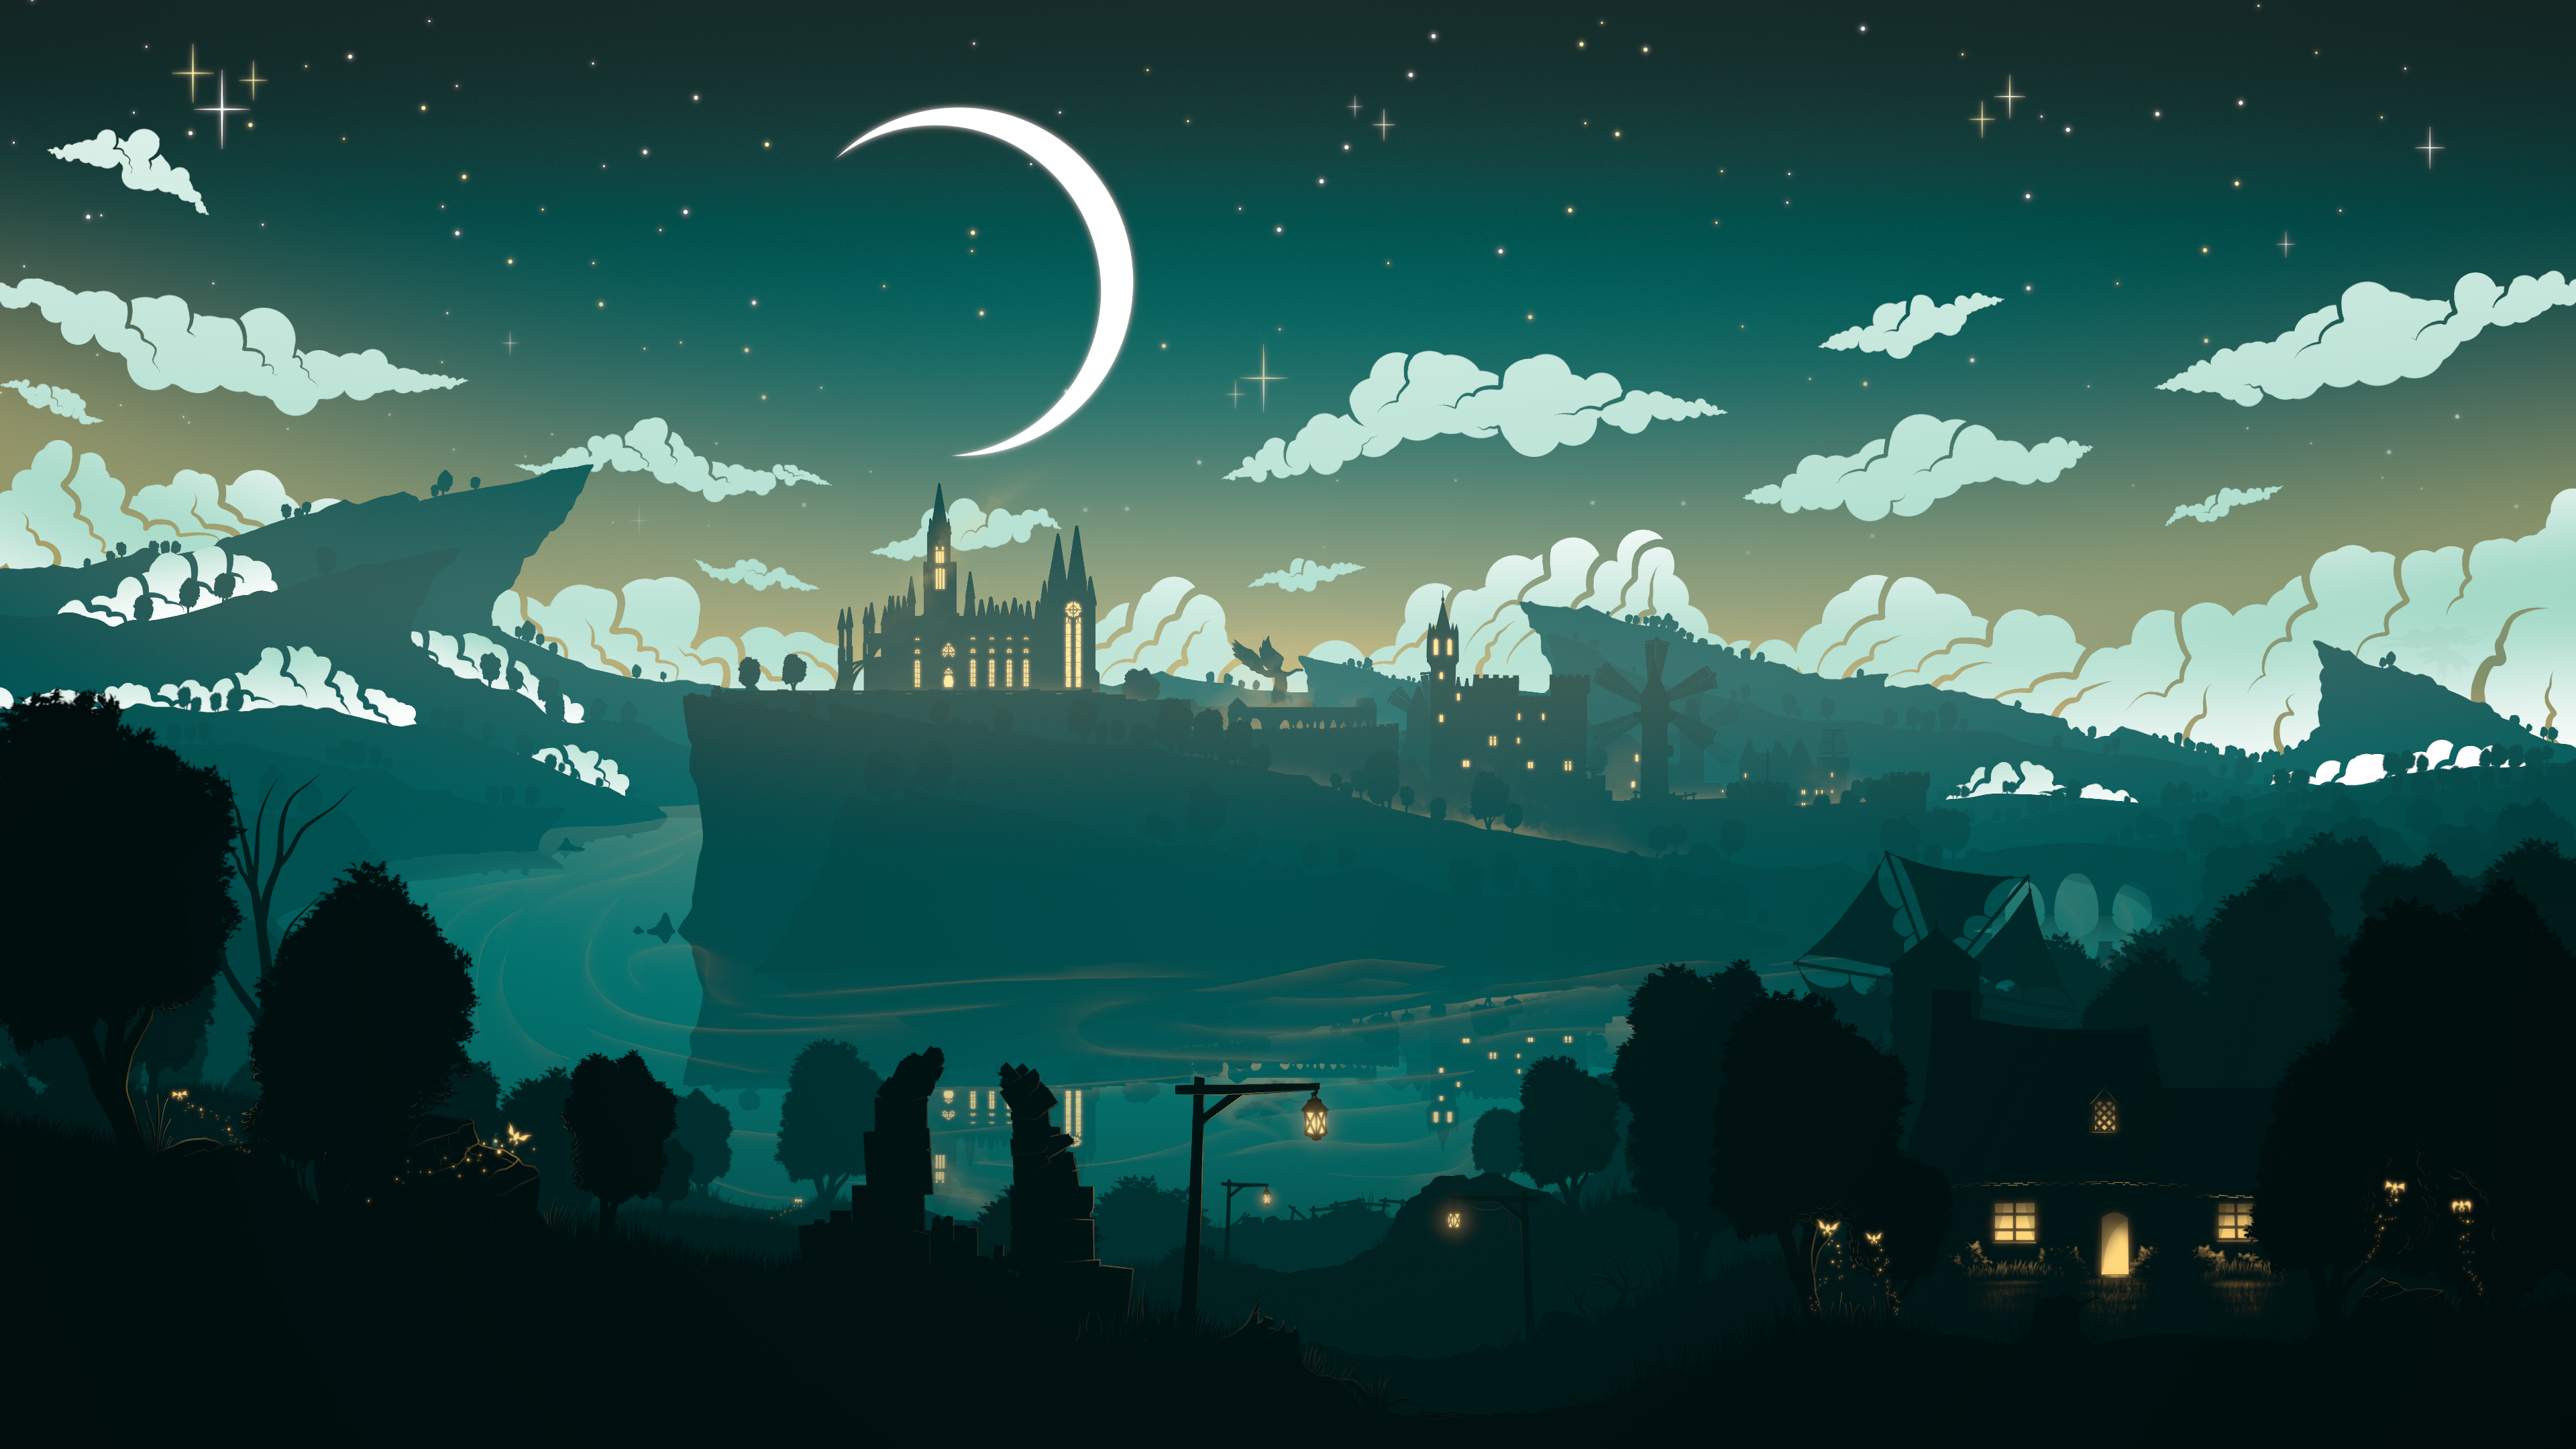
\includegraphics[height=\linewidth]{./pics/8.png}}
}
\vspace*{2em}
\begin{center}
    \color{white}
    \scale{6}{utarticle文档类介绍}
\end{center}

\vfill
\hspace*{35em}\textcolor{white}{\huge Date\;:\;\today}

\vspace*{1em}
\hspace*{35em}\textcolor{white}{\huge 作者\;:\;Eureka}




\clearpage
\section{基本结构}
\subsection{字体控制}
    
{\ttfamily 我第二次到仙岩的时候,我惊诧于梅雨潭的绿了。梅雨潭是一个瀑布潭。
仙瀑有三个瀑布,梅雨瀑最低。走到山边,便听见花花花花的声音;
抬起头,镶在两条湿湿的黑边儿里的,一带白而发亮的水便呈现于眼前了。
我们先到梅雨亭。梅雨亭正对着那条瀑布}

\textit{坐在亭边,不必仰头,便可见它的全体了。
亭下深深的便是梅雨潭。这个亭踞在突出的一角的岩石上,上下都空空儿的;
仿佛一只苍鹰展着翼翅浮在天宇中一般。}

\textbf{那溅着的水花,晶莹而多芒;
远望去,像一朵朵小小的白梅,微雨似的纷纷落着。据说,这就是梅雨潭之所以得名了。
但我觉得像杨花,格外确切些。}


\subsection{批注设置}
轻风起来时,点点随风飘散,那更是杨花了——这时偶然有几点送入我们温暖的怀里,便倏的钻了进去,再也寻它不着。
三面都是山,像半个环儿拥着;人如在井底了。这是一个秋季的薄阴的天气。在\verb|withgezhu|环境中,
{\bfseries 使用|\{《你的割注内容》\}}开始割注。下面演示一个示例:

\begin{withgezhu}
割注开始
\begingroup
\color{blue}
|{微微的云在我们顶上流着;岩面与草丛都从润湿中透出几分油油的绿意。而瀑布也似乎分外的响了。
那瀑布从上面冲下,仿佛已被扯成大小的几绺}
\endgroup 
割注结束
\end{withgezhu}

{\kaishu 不复是一幅整齐而平滑的布。岩上有许多棱角;瀑流经过时,作急剧的撞击,便飞花碎玉般乱溅着了。}

\subsection{注意}
其中一个需要注意的问题就是:{\bfseries 亚洲文字几乎都是会倒过来的,但是西文或者进一步说就是ASCII符号,或单词是不会旋转的}。

而且我们可以使用脚注\footnote[1]{当然有一个东西叫做行间注,需要一个专门的\texttt{pxrubrica}宏包},
和之前的语法是一样的,使用命令\verb|footnote|即可.这是一段正文,在这段正文中添加行间注\footnote[2]{这是脚注的内容}。



\clearpage
\section{Math Formula}
\subsection{行内公式}
这里用于测试数学公式环境:行内公式测试,这里使用了一个常用的公式:$a^2 + b^2 = c^2$。


\subsection{行间公式}
行间公式测试,这里首先使用常用的\verb|\[\]|环境:
\[
    \sum_{i=1}^{+\infty}{\frac{1}{i^2}} = \frac{\pi^2}{6}
\]

然后再测试以下\verb|amsmath|宏包,为了让公式的编号易于识别,我把公式的编号进行了旋转$90^\circ$操作。
具体的使用效果如下:
\begin{align}
    \sum_{i=1}^{+\infty}{\frac{1}{i^2}} = \frac{\pi^2}{6}
\end{align}

\subsection{大型公式}
本模板定义了一个旋转align环境\verb|ralign|,可以指定它的公式宽度,默认\verb|.2\linewidth|。效果如下:
\begin{ralign}[.5\linewidth]
    \lim _{\Delta x \rightarrow 0} \frac{1}{\sqrt[3]{x}} & =\lim _{\Delta x \rightarrow 0} \frac{\frac{1}{\sqrt[3]{x+\Delta x}}-\frac{1}{\sqrt[3]{x}}}{\Delta x} \\
    & =\frac{x}{\Delta x}\left(\frac{\frac{-\Delta x}{x(x+\Delta x)}}{\frac{1}{\sqrt[3]{(x+\Delta x)^{2}}}+\frac{1}{\sqrt[3]{(x(x+\Delta x))}}+\frac{1}{\sqrt[3]{x^{2}}}}\right) \\
    & =\frac{-\frac{x}{x^{2}}}{\frac{1}{3 \sqrt[3]{x^{2}}}}=-\frac{1}{3} x^{-\frac{1}{3}}
\end{ralign}

\subsection{切为正常模式}
如果你想要切换为平时的正常模式可以使用\verb|latex|自带的\verb|lscape|宏包。
下面即为一个演示:
\begin{landscape}
    This page is in landscape mode. 我们可以在这一页添加我们不方便表达的任何内容。

    \begin{align}
        \sum_{i=1}^{+\infty}{\frac{1}{i^2}} = \frac{\pi^2}{6}
    \end{align}

    Although the Chinese font isn't working properly, but the Math formula working.

    \vspace*{5em}
    \begin{figure}[!htb]
        \centering
        \includegraphics[scale=.15, angle=-90]{./pics/017.png}
        \caption{旋转图片}
        \label{旋转图片}
    \end{figure}
\end{landscape}


\clearpage
\section{fig insert}
为了在uplatex编译的utarticle中插入图片,在引入\verb|graphicx|宏包时应该更改为:
\verb|\usepackage[dvipdfmx]{graphicx}|,不然会报错:
\verb|LaTeX Error: Cannot determine size of graphic in <file_pic>|
{\bfseries 原因:}更改后的这种方式适用于使用传统的latex编译命令,通过dvipdfmx命令将生成的DVI文件转换为PDF文件。

然而原始的\verb|\usepackage{graphicx}|方式适用于:\verb|pdflatex,xelatex, lualatex|

同理,对应的adjustbox宏包也应该指定\verb|dvips|选项,不然就不能够正常显示\verb|.jpg, .png|的图片。

\vspace*{5em}
\begin{figure}[!htb]
    \centering
    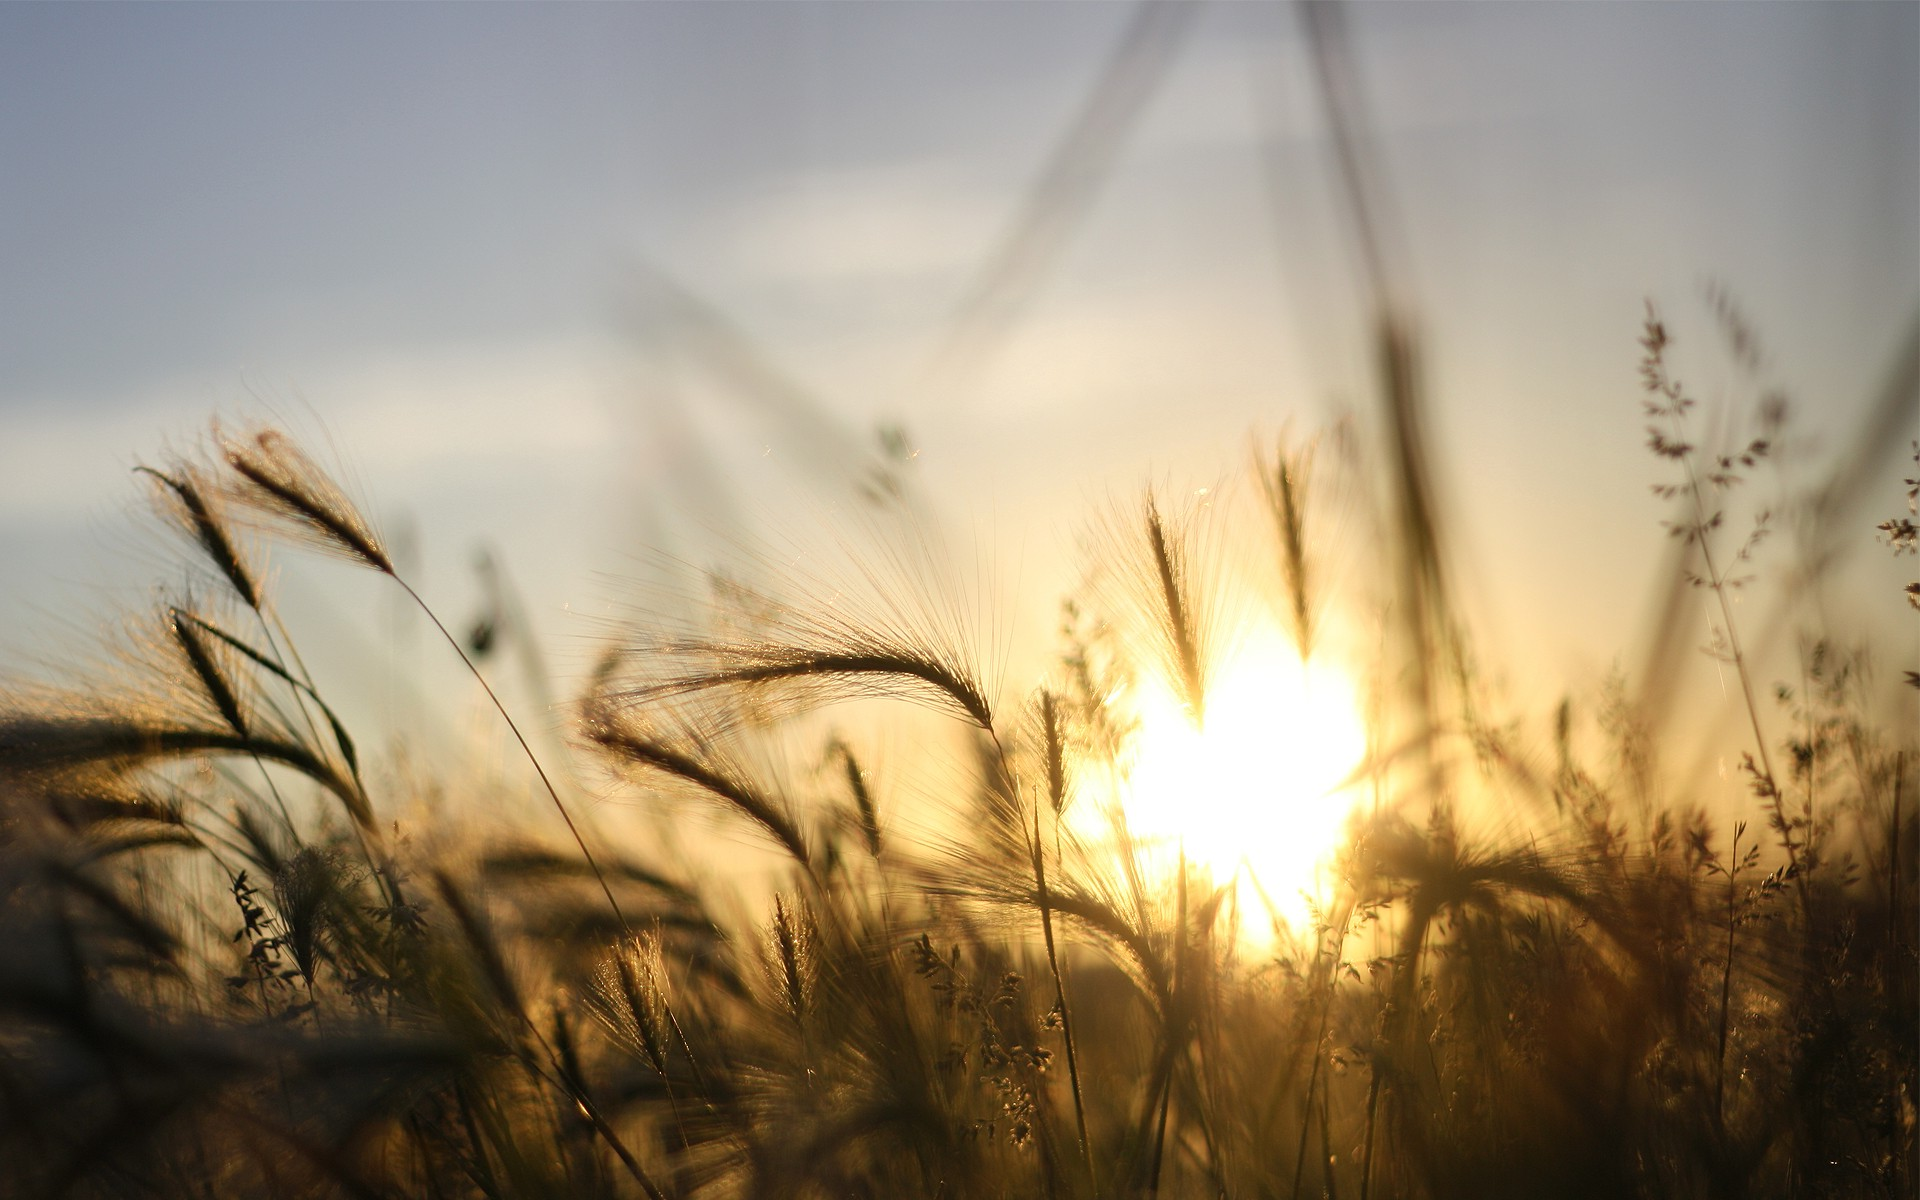
\includegraphics[scale=.1]{./pics/wheat.jpg}
    \hspace*{10em}
    
\includegraphics[scale=.35]{./pics/GNU_logo.pdf}
    \caption{图片插入测试}
    \label{图片插入测试}
\end{figure}


\clearpage
\thispagestyle{empty}
\begingroup
\color{white} 
\subsection{背景图片}
% 在特定页面添加背景图片
\AddToShipoutPictureBG*{%
    \AtPageLowerLeft{
\includegraphics[height=\linewidth]{./pics/020.png}}
}

为了引入图片作为背景,本模板使用了宏包\verb|eso-pic|,这个宏包相比于\verb|background|宏包更加的灵活,
可以指定某一页的背景,而\verb|background|宏包则只能指定全局的背景。

由于\verb|utarticle|文档类倒过来了,于此时图片的高(此时的横向距离)是原来的宽.
同时我们制定了图片的anchor为页面的左下角。


\vspace*{10em}
\section{结语}
\begin{center}
    \scale{8}{Thanks}
\end{center}


\endgroup

\end{document}
